\chapter{Background}

This chapter introduces the necessary concepts... %
\autoref{sec:mc} describes... %

For the complete syntax, please refer to the Btor2 publication~\cite{btor2}

\todoZs{Summarize bg}

\section{Model Checking}\label{sec:mc}

The challenge of verifying programs without executing or deploying them has been a central research topic since the late 20\textsuperscript{th} century~\cite{systemEngineering}. One of the principal approaches addressing this problem is \textit{formal verification}, which aims to provide mathematically rigorous proofs for the correct operation of computer programs~\cite{MC}.

Among formal verification techniques, \textit{model checking}~\cite{modelChecking, modelChecking2} has become one of the most widely used and practically applicable methods. Given a software or hardware system, model checking systematically and exhaustively explores all possible executions for every possible input to determine whether specified properties hold. Unlike testing or simulation, which inspects only a limited subset of behaviors, model checking offers \textbf{exhaustive verification} -- meaning if a property is satisfied, it holds for all possible executions of the model; if it is violated, the model checker produces a \textbf{counterexample} that reflects an actual execution leading to an error state.

Model checking provides an automated means of verifying concurrent, finite-state systems by performing an efficient symbolic or explicit traversal of the system's \textbf{state space}. Each state represents a possible configuration of the system's variables, and transitions between states correspond to execution steps. The model checker evaluates whether temporal logic properties, such as safety and liveness constraints, hold over this state graph.~\cite{hardware_MC}

Typical properties include detecting \textit{assertion violations}, \textit{out-of-bounds indexing}, and \textit{arithmetic overflows}. In this work, the focus is primarily on the \textbf{reachability property}, which concerns determining whether a given “bad” or error state is reachable from the initial configuration of the system. Demonstrating that no such state can be reached constitutes a proof of safety for the given model.

While model checking is powerful, it suffers from the well-known \textbf{state-space explosion problem}~\cite{statespaceexplosionproblem}. The number of possible states grows exponentially with the number of variables in the system. For example, a program with three 32-bit input variables already has
\[
2^{32} \cdot 2^{32} \cdot 2^{32} = 2^{96}
\]
possible input combinations, making exhaustive exploration computationally infeasible for large-scale systems. This challenge has motivated extensive research into more scalable techniques, such as symbolic model checking~\cite{symbolicMC}, abstraction and refinement methods\cite{boundedMC}, and SAT-based~\cite{SMT-LIB} approaches like IC3~\cite{ic3}.

\section{Control-Flow Automata}\label{sec:cfa}

Many programming languages tend to have ambiguities and complex structures that may help the developers express themselves more concisely, but are hard to handle in low-level algorithms. For this purpose input programs must be transformed into a simplified formal representation that accurately captures their behaviour. Common high-level forms of these models include transition systems, which describe states and their possible transitions, and automata, which represent system behavior through states and input-driven transitions.

To perform this transformation, software model checking toolchains typically employ specialized frontends that translate the source code into these formal models, so the so called "backend" can analyze it and apply mathematical and algorithmic reasoning to system properties in a precise and efficient way.

A widely used formalism is the \textbf{Control-Flow Automata (CFA)}~\cite{cfa}, which is formally defined as:

\noindent\textbf{Definition \label{def:cfa}(Control-flow automata).} 
A control-flow automaton is a tuple 
\[
\textit{CFA} = (V, L, l_0, E)
\]
where
\begin{itemize}
  \item $V = \{v_1, v_2, \ldots, v_n\}$ is a set of variables with domains $D_{v_1}, D_{v_2}, \ldots, D_{v_n}$,
  \item $L$ is a set of program \textit{locations} modeling the program counter,
  \item $l_0 \in L$ is the \textit{initial} program location (entry point),
  \item $E \subseteq L \times Ops \times L$ is a set of directed \textit{edges} representing the \textit{operations} that are executed when control flows from the source location to the target. $ Ops $ can either be \textit{assignments} or \textit{assumptions}. Assignments change a single variable -- there is a special case called \textit{havoc}, which is a nondeterministic assignement -- and assumptions check a condition.
\end{itemize}

\begin{figure}
  \centering
  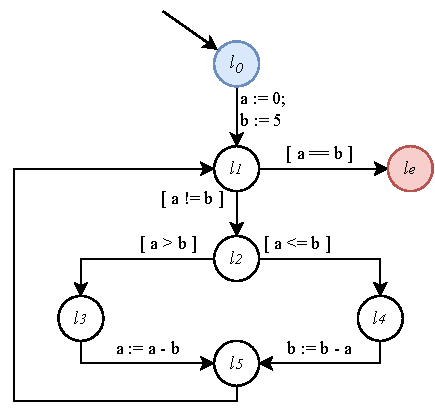
\includegraphics[width=0.5\textwidth]{figures/cfa_simple.drawio.pdf}
  \caption{Simple representation of a Control-Flow Automata (CFA).}
  \label{fig:cfa}
\end{figure}

Figure~\ref{fig:cfa} illustrates a simple control-flow automaton (CFA). The blue location $l_0$ denotes the \textit{initial state} of the program. It is important to distinguish between \textit{states} and \textit{locations} in the context of CFAs. In this example, there are two variables, $a$ and $b$, each assigned a value. Together, these values define a \textit{concrete data state}. If the variables instead represented sets of possible values determined by the program's constraints, they would form \textit{abstract states}.

The red location represents the \textit{error location}, which corresponds to an unsafe program state. A \textit{counterexample} demonstrates a feasible path from an initial state to such an unsafe state, whereas a proof of safety ensures that no unsafe state is ever reachable. Although reachability queries can, in principle, treat any state as unsafe, it is common to restrict these to specific \textit{unsafe locations}, since program specifications are often expressed as assertions in the code.

An execution of the program corresponds to a \textit{concrete trace} -- a sequence of concrete states and transitions within the CFA's state space. These traces can be projected onto the graph defined by the CFA's locations and edges to form directed paths, which correspond to specific executions of the program.

In contrast, an \textit{abstract trace} consists of abstract states and transitions within an abstraction of the state space. Abstract traces do not always correspond to real program executions. An abstract trace is considered \textit{feasible} if, when applying the transition effects to each abstract state, the resulting states remain consistent with the target abstract states. Otherwise, the trace is \textit{infeasible}. Feasibility thus depends on whether there exists a corresponding concrete trace that follows the same path and satisfies all the constraints of the abstract states.


\section{The Hardware Model Checking Format BTOR2}\label{sec:btor2}

Hardware model checking is a verification technique used to ensure that digital hardware designs behave correctly according to their specifications. It has been a long-established and highly successful application domain within formal methods, with early breakthroughs such as bounded model checking (BMC) \cite{boundedMC} demonstrating the practicality of applying SAT- and SMT-based reasoning to hardware verification problems.

In this domain, the goal is to check whether a hardware model -- typically represented as a sequential circuit -- satisfies certain logical properties. A sequential circuit is a digital system composed of combinational logic (which determines outputs based solely on current inputs) and memory elements such as flip-flops or registers (which store the system's state across clock cycles). Verification then involves exploring the circuit's possible state transitions over time to ensure that unsafe or undesired (\verb|bad|) states are never reachable. In the context of model-checking that is called \textit{reachability safety}.

% Btor2: 
% what is it (and maybe try to explain in 1-2 sentences what all the words in it's description mean)
% AIGER successor
% HWMCC: what is HWMCC; it uses btor2 as official format
% btor2 example
% add a subsection on sorts, and maybe mention that we will focus on bitvectors only in this work

The Hardware Model Checking Competition (HWMCC)~\cite{hwmcc} serves as a benchmark for evaluating formal verification tools for hardware systems. A key innovation supporting this effort is BTOR2~\cite{btor2}, a word-level model checking format designed for bit-precise modeling of word-level sequential circuits.
The BTOR2 language extends the previous bit-level AIGER~\cite{AIGER} format with higher-level abstractions, making it ideal for various verification techniques. It introduces a simple, sorted, line-based syntax that is easy to parse and aligns with SMT-LIB~\cite{SMT-LIB} semantics for bit-vectors and arrays.

\subsection{Syntax of BTOR2}

The BTOR2 language identifies 2 entities called \textit{sort} and \textit{node}. Each line of code starts with a number, respectively \verb|sid| (sort id) and \verb|nid| (node id) which can be referenced in the subsequent lines.  

A \emph{sort} can be one of two types: a bit-vector of arbitrary width~$w$, denoted by~$\mathcal{B}^w$, or an array type. An array type is expressed as~$\mathcal{A}^{I \to E}$, where~$I$ and~$E$ are bit-vector types representing the index and element sorts, respectively.

A \emph{node} may correspond to an \emph{input}, a \emph{state}, or the \emph{result} of applying an operator to other nodes. Inputs represent external signals provided to the BTOR2 circuit, while states correspond to the circuit's memory elements. Typically, inputs have bit-vector types, whereas states may be either bit-vector or array types. In this report I will only focus on the bit-vector cases.

Operators serve as the fundamental building blocks of a BTOR2 circuit. Each operator takes arguments of specific types and produces a result of a well-defined type. The general syntax for defining a BTOR2 operator is:

\[
\langle \text{nid} \rangle\ \langle \text{op} \rangle\ \langle \text{sid} \rangle\ \langle \text{nid}_1 \rangle\ [\langle \text{nid}_2 \rangle\ [\langle \text{nid}_3 \rangle]]
\]

This notation specifies that the node identified by \verb|nid| stores the result of applying the operator~\verb|op| to one, two, or three operands. The resulting node has type~\verb|sid| and can be referenced by its identifier.

{BTOR} also includes constructs such as \texttt{init}, \texttt{next}, and \texttt{bad} for describing safety and reachability properties of sequential circuits. The \texttt{init} keyword defines initial states, while \texttt{bad} identifies unsafe or error states. The \texttt{next} construct specifies state transitions between consecutive time steps.

\subsubsection{Count2 Example}

\definecolor{backcolour}{rgb}{0.95,0.95,0.92}

\lstdefinestyle{mystyle}{
  backgroundcolor=\color{backcolour}, 
  basicstyle=\ttfamily\footnotesize,
  breakatwhitespace=false,         
  breaklines=true,                 
  captionpos=b,                    
  keepspaces=true,                 
  numbers=left,                    
  numbersep=5pt,
  numberstyle=\ttfamily\footnotesize, 
  frame=none,                                       
  showspaces=false,                
  showstringspaces=false,
  showtabs=false,                  
  tabsize=2
}

\lstset{style=mystyle}
\begin{lstlisting}[language=Verilog, 
  caption=BTOR2 example,
  label={list:btor2}]
; source: https://github.com/Boolector/btor2tools/tree/b8456dda4780789e882f5791eb486f295ade4da4/examples/btorsim
1 sort bitvec 3
2 zero 1
3 state 1
4 init 1 3 2
5 one 1
6 add 1 3 5
7 next 1 3 6
8 ones 1
9 sort bitvec 1
10 eq 9 3 8
11 bad 10
\end{lstlisting}

In \autoref{list:btor2} is a BTOR2 circuit that defines a simple finite state machine -- a 3-bit counter -- that starts from zero and increments by one at each time step. Each line defines a node in the circuit, such as a constant, state, operation, or property.

% \todoZs{I would put this whole thing into a description (\url{https://www.overleaf.com/learn/latex/Lists\#The\_description\_environment}), where each label is "Node x" or something like that - whatever looks good and makes sense}

% At the beginning of the circuit, line 1 declares a bit-vector of width 3 \verb|sort bitvec 3|, which serves as the type for all 3-bit values used throughout the circuit. This will have a sort id or \verb|sid| of '1' which will be used to declare registers and operations.

% Line 2 defines a constant zero \verb|zero 1|, which produces the bit-vector \verb|000| and has a node id or \verb|nid| of '2'. Following this, line 3 introduces a state variable of sort 1 (3 bits), representing the main state of the circuit.

% The initial value of state '3' is specified in line 4, which uses the init keyword to bind state 3 to start at constant 2, which is the \verb|000| bit-vector. The next input is defined in line 5 using one 1, which denotes the constant \verb|001|.

% Line 6 defines an addition operation that adds 1 to the main state, resulting in node 6, the next value of the counter. This operation wraps around on overflow due to the fixed 3-bit width. Line 7 then uses the next keyword to specify that in the next state, the counter should take the value of node 6, i.e., the incremented result.

% To define a property of interest, line 8 declares another constant: \verb|ones 1|, which represents the maximum value a 3-bit counter can hold—namely \verb|111|. Line 9 introduces a new sort of width 1, which is used for boolean-like signals such as equality checks.

% Line 10 defines a comparison between the current counter value and the maximum value \verb|111| using the eq operator. This operation returns a 1-bit result: true (1) if the counter is at maximum, false (0) otherwise. Finally, line 11 marks this equality result as a bad state, which is a safety property violation. Hence, the circuit asserts that reaching the value 111 is undesirable or erroneous.

% \todoZs{I'll go through the description of the example when it's made into a description}

% In summary, this BTOR2 circuit models a 3-bit counter that increments with each step and triggers a bad state when it reaches 111. This design could be used in formal verification to prove that the system avoids overflow, or alternatively, to find the point at which it does. The clear structure and modular nature of BTOR2 make it suitable for such sequential hardware modeling and property checking.

% \subsection{Btor2C}

% \todoZs{structure in latex comments}
% % what is Btor2C, what does it do
% % why is it useful (in a bit more detail? see abstract, I think we talked about this more there, maybe not in the final version, idk)
% % an example of a C program from a btor2 circuit (C can be simplified, just mention that)

% Btor2C~\cite{btor2c} is a tool that translates Btor2 hardware models into equivalent C programs. This allows software verification tools to analyze hardware designs, bridging the gap between hardware and software verification.
% \todoZs{you don't need to talk about your work yet - the reader has no idea what your implementation is yet anyways - but that's for later} In my implementation, I focused on bit-vectors and their related functions and definitions, leveraging the expressive power of BTOR2 to model and verify small, bit-precise sequential systems.

% \todoZs{So far it was clear what we need to introduce - but jumping to Theta next seems to make a hole here to me - we will need to think about what else needs to be introduced - but maybe do that while starting to write the next chapter(s) - I think a lot of stuff will come up}
